\begin{task}

\TT{Wyznacz udział mocy podstawowej (pierwszej) harmonicznej w całkowitej mocy okresowego sygnału $f(t)$ przedstawionego na rysunku:}{Compute the percentage contribution of the fundamental (first) harmonic in the total power of the periodic square signal shown in the figure below:} 

\begin{figure}[H]
\centering
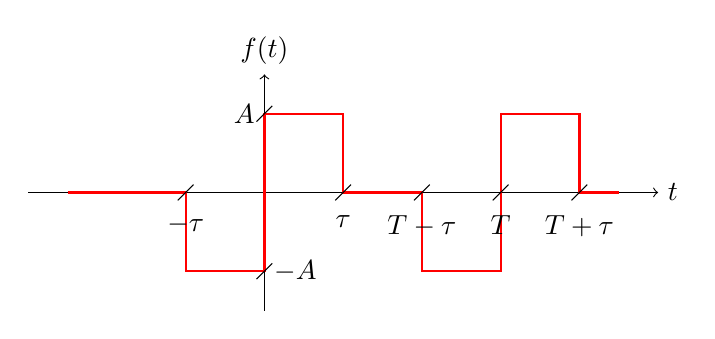
\begin{tikzpicture}
  %\draw (0,0) circle (1in);
  \draw[->] (-3.0,+0.0) -- (+5.0,+0.0) node[right] {$t$};
  \draw[->] (+0.0,-1.5) -- (+0.0,+1.5) node[above] {$f(t)$};
  \draw[-,red, thick] (-2.5,+0.0) -- (-1.0,+0.0) -- (-1.0,-1.0) --(+0.0,-1.0) -- (+0.0,+1.0) -- (+1.0,+1.0) -- (+1.0,+0.0) -- (+2.0,+0.0) -- (+2.0,-1.0) -- (3.0,-1.0) -- (3.0,1.0) -- (4.0,1.0) -- (4.0,0.0) -- (4.5,0.0);
  \draw[-] (-1.0-0.1,-0.1)--(-1.0+0.1,0.1) node[midway, below, outer sep=5pt,align=center] {$-\tau$};
  \draw[-] (+1.0-0.1,-0.1)--(+1.0+0.1,0.1) node[midway, below, outer sep=5pt] {$\tau$};
  \draw[-] (+2.0-0.1,-0.1)--(+2.0+0.1,0.1) node[midway, below, outer sep=5pt] {$T-\tau$};
  \draw[-] (+3.0-0.1,-0.1)--(+3.0+0.1,0.1) node[midway, below, outer sep=5pt] {$T$};
  \draw[-] (+4.0-0.1,-0.1)--(+4.0+0.1,0.1) node[midway, below, outer sep=5pt] {$T+\tau$};
  \draw[-] (-0.1,1.0-0.1)--(+0.1,1.0+0.1) node[midway, left] {$A$};
  \draw[-] (-0.1,-1.0-0.1)--(+0.1,-1.0+0.1) node[midway, right] {$-A$};
\end{tikzpicture}
\end{figure}

\begin{equation}
\frac{P_1}{P} = ?
\end{equation}

\TT{W pierwszej kolejności należy opisać sygnał za pomocą wzoru:}{First of all, the definition of $f(t)$ signal has to be derived. This is periodic piecewise linear function, which may be describe as:}

\begin{equation}
f(t)=\begin{cases}-A & t \in \left ( -\tau+k \cdot T; 0 +k \cdot T\right )\\
A & t \in \left (  0+k \cdot T; \tau + k \cdot T \right ) \end{cases} \wedge k \in \TT{C}{Z}
\end{equation}

\TT{Moc sygnału możemy obliczyć ze wzoru:}{The total power of the signal is defined as:}

\begin{equation}
	P=\frac{1}{T} \cdot \int_{T}^{}\left|f(t)\right|^2 \cdot dt
\end{equation}

\TT{Podstawiając wartości sygnału $f(t)$ do wzoru na moc otrzymujemy:}{For the period $t \in (0; T)$, i.e. $k=0$, we get:}

\begin{align*}
P &=\frac{1}{T} \cdot \int_{T}\left|f(t)\right|^2 \cdot dt=\\
&=\frac{1}{T} \cdot \left( \int_{-\tau}^{0} \left|-A\right|^2 \cdot dt + \int_{0}^{\tau} \left|A\right|^2 \cdot dt \right)=\\
&=\frac{1}{T} \cdot \left( A^2 \cdot \int_{-\tau}^{0} dt + A^2 \cdot \int_{0}^{\tau} dt  \right)=\\
&=\frac{A^2}{T} \cdot \left( \left. t\right |_{-\tau}^{0} + \left. t\right|_{0}^{\tau} \right)=\\
&=\frac{A^2}{T} \cdot \left( 0 - (-\tau) + \tau - 0\right)=\\
&=\frac{A^2}{T} \cdot \left( 2 \cdot \tau \right)=\\
&=\frac{2 \cdot A^2 \cdot \tau}{T} 
\end{align*}

\TT{Moc sygnału $f(t)$ równa się $\frac{2 \cdot A^2 \cdot \tau}{T}$.}{The total power of the $f(t)$ signal equals $\frac{2 \cdot A^2 \cdot \tau}{T}$.}

\TT{Moc podstawowej (pierwszej) harmonicznej to (na podstawie twierdzenia Parsevala):}{Based on Parseval theorem, power of the fundamental harmonic is defined as:}

\begin{equation}
	P_1=\left|F_{1}\right|^2+\left|F_{-1}\right|^2
\end{equation}

\TT{Ponieważ sygnał $f(t)$ jest sygnałem rzeczywistym, to $\left|F_{1}\right|=\left|F_{-1}\right|$, czyli moc podstawowej harmonicznej:}{Because the $f(t) \in R$, thus $\left|F_{1}\right|=\left|F_{-1}\right|$ and the power of the fundamental harmonic may be calculated as}

\begin{equation}
	P_1=2 \cdot \left|F_{1}\right|^2
\end{equation}

\TT{W związku z tym, należy obliczyć wartość współczynnika $F_1$. Można to zrobić bezpośrednio ze wzoru na $F_k$ podstawiając $k=1$:}{In order to calculate the $P_1$, the $F_1$ coefficient has to be calculated:}

\begin{equation}
	F_1=\frac{1}{T} \cdot \int_{T}f(t) \cdot e^{-\jmath \cdot \frac{2\pi}{T} \cdot t} \cdot dt
\end{equation}

\TT{Podstawiając wartości sygnału $f(t)$ do wzoru na $F_1$ otrzymujemy:}{For the period $t \in (0; T)$, i.e. $k=0$, we get:}

\begin{align*}
F_1&=\frac{1}{T} \cdot \int_{T}f(t) \cdot e^{-\jmath \cdot \frac{2\pi}{T} \cdot t} \cdot dt=\\
&=\frac{1}{T} \cdot \left(\int_{-\tau}^{0}-A \cdot e^{-\jmath \cdot \frac{2\pi}{T} \cdot t} \cdot dt + \int_{0}^{\tau}A \cdot e^{-\jmath \cdot \frac{2\pi}{T} \cdot t} \cdot dt\right)=\\
&=\frac{-A}{T} \cdot \left(\int_{-\tau}^{0}e^{-\jmath \cdot \frac{2\pi}{T} \cdot t} \cdot dt - \int_{0}^{\tau}e^{-\jmath \cdot \frac{2\pi}{T} \cdot t} \cdot dt\right)=\\
&=\begin{Bmatrix*}[l]
z&=-\jmath \cdot \frac{2\pi}{T} \cdot t\\
dz&=-\jmath \cdot \frac{2\pi}{T} \cdot dt\\
dt&=\frac{dz}{-\jmath \cdot \frac{2\pi}{T}}\\
\end{Bmatrix*}=\\
&=\frac{-A}{T} \cdot \left(\int_{-\tau}^{0} e^{z} \cdot \frac{dz}{-\jmath \cdot \frac{2\pi}{T}}-\int_{0}^{\tau} e^{z} \cdot \frac{dz}{-\jmath \cdot \frac{2\pi}{T}}\right)=\\
&=\frac{A}{T \cdot \jmath \cdot \frac{2\pi}{T}} \cdot \left(\int_{-\tau}^{0} e^{z} \cdot dz - \int_{0}^{-\tau} e^{z} \cdot dz\right)=\\
&=\frac{A}{\jmath \cdot 2 \pi} \cdot \left(\left. e^{z} \right|_{-\tau}^{0} - \left. e^{z} \right|_{0}^{\tau}\right)=\\
&=\frac{A}{\jmath \cdot 2 \pi} \cdot \left(\left. e^{-\jmath \cdot \frac{2\pi}{T} \cdot t} \right|_{-\tau}^{0} - \left. e^{-\jmath \cdot \frac{2\pi}{T} \cdot t} \right|_{0}^{\tau}\right)=\\
&=\frac{A}{\jmath \cdot 2 \pi} \cdot \left( e^{-\jmath \cdot \frac{2\pi}{T} \cdot 0} - e^{-\jmath \cdot \frac{2\pi}{T} \cdot (-\tau)} -e^{-\jmath \cdot \frac{2\pi}{T} \cdot \tau} + e^{-\jmath \cdot \frac{2\pi}{T} \cdot 0}\right)=\\
&=\frac{A}{\jmath \cdot 2 \pi} \cdot \left( e^{0} - e^{\jmath \cdot \frac{2\pi}{T} \cdot \tau} -e^{-\jmath \cdot \frac{2\pi}{T} \cdot \tau}+e^{0}\right)=\\
&=\frac{A}{\jmath \cdot 2 \pi} \cdot \left( 1 - e^{\jmath \cdot \frac{2\pi}{T} \cdot \tau} -e^{-\jmath \cdot \frac{2\pi}{T} \cdot \tau}+1\right)=\\
&=\frac{A}{\jmath \cdot 2 \pi} \cdot \left( 2 - \left(e^{\jmath \cdot \frac{2\pi}{T} \cdot \tau} +e^{-\jmath \cdot \frac{2\pi}{T} \cdot \tau}\right)\right)=\\
&=\begin{Bmatrix}
\EulerCos
\end{Bmatrix}=\\
&=\frac{A}{\jmath \cdot 2 \pi} \cdot \left( 2 - 2 \cdot cos\left(\frac{2\pi}{T} \cdot \tau\right)\right)=\\
&=\frac{A}{\jmath \cdot \pi} \cdot \left( 1 - cos\left(\frac{2\pi}{T} \cdot \tau\right)\right)=\\
&=\jmath \cdot \frac{A}{\pi} \cdot \left(cos\left(\frac{2\pi}{T} \cdot \tau\right) -1 \right)
\end{align*}

\TT{Wartość współczynnika $F_1$ to $\jmath \cdot \frac{A}{\pi} \cdot \left(cos\left(\frac{2\pi}{T} \cdot \tau\right) -1 \right)$}{The $F_1$ coefficient equals $\jmath \cdot \frac{A}{\pi} \cdot \left(cos\left(\frac{2\pi}{T} \cdot \tau\right) -1 \right)$.}

\TT{Podstawiając wartość współczynnika $F_1$ do wzoru na moc podstawowej harmonicznej otrzymujemy:}{Thus, the $P_1$ may be calculated:}

\begin{align*}
P_1&=2 \cdot \left|F_{1}\right|^2=\\
&=2 \cdot \left|\jmath \cdot \frac{A}{\pi} \cdot \left(cos\left(\frac{2\pi}{T} \cdot \tau\right) -1 \right)\right|^2=\\
&=2 \cdot \left[\frac{A}{\pi} \cdot \left(cos\left(\frac{2\pi}{T} \cdot \tau\right) -1 \right)\right]^2=\\
&=\frac{2 \cdot A^2}{\pi^2} \cdot \left[cos\left(\frac{2\pi}{T} \cdot \tau\right) -1 \right]^2
\end{align*}

\TT{Moc podstawowej harmonicznej równa się $P_1=\frac{2 \cdot A^2}{\pi^2} \cdot \left[cos\left(\frac{2\pi}{T} \cdot \tau\right) -1 \right]^2$.}{The power of the fundamental harmonic equals $P_1=\frac{2 \cdot A^2}{\pi^2} \cdot \left[cos\left(\frac{2\pi}{T} \cdot \tau\right) -1 \right]^2$.}

\TT{Teraz można wyznaczyć udział mocy podstawowej (pierwszej) harmonicznej w całkowitej mocy okresowego sygnału $f(t)$:}{Finally, the percentage contribution of the fundamental harmonic in the total power of the $f(t)$ signal is equal to:}

\begin{equation}
	\frac{P_1}{P} = \frac{\frac{2 \cdot A^2}{\pi^2} \cdot \left[cos\left(\frac{2\pi}{T} \cdot \tau\right) -1 \right]^2}{\frac{2 \cdot A^2 \cdot \tau}{T}}=\frac{T}{\pi^2 \cdot \tau} \cdot \left[cos\left(\frac{2\pi}{T} \cdot \tau\right) -1 \right]^2
\end{equation}

\begin{figure}[H]
	\centering
	\begin{tikzpicture}
		%\draw (0,0) circle (1in);
		\draw[->] (-0.5,+0.0) -- (+5.0,+0.0) node[right] {$\tau$};
		\draw[->] (+0.0,-0.5) -- (+0.0,+1.5) node[above] {$\frac{P_1}{P}$};
		\draw[-] (+4.0-0.1,-0.1)--(+4.0+0.1,0.1) node[midway, below, outer sep=5pt] {$\frac{T}{2}$};

		\draw[-] (-0.1,0.81-0.1)--(+0.1,0.81+0.1) node[midway, left] {$\frac{8}{\pi^2}$};
		
		\draw[scale=1.0,domain=0.01:4.0,samples=100,smooth,variable=\x,red,thick] plot ({\x},{2*1/(3.141592*3.141592*\x/4)*(cos(\x*180.0/4)-1)*(cos(\x*180.0/4)-1)});
	\end{tikzpicture}
\end{figure}
%plot({\x},{1/(3.141592*3.141592*\x)*(cos(180.0*2*\x)-1)*(cos(180.0*2*\x)-1)});

\end{task}